\documentclass[12pt, a4paper]{article}

\usepackage[czech]{babel}
\usepackage[IL2]{fontenc}
\usepackage[utf8]{inputenc}
\usepackage{lmodern}  % lepší kvalita PDF

\usepackage[a4paper,top=3cm,bottom=3cm,left=3cm,right=3cm,marginparwidth=1.75cm]{geometry}

\usepackage{graphicx}
\usepackage{titling}
\usepackage{enumitem}
\usepackage{caption}
\usepackage{float}
\usepackage{pdfpages}
\usepackage{verbatim}
\usepackage{amsmath}

\usepackage{pkg-custom-commands}
\usepackage{pkg-url}

% údaje na titulní straně
\title{Cvičení 3}
\def \thesubtitle {KIV/VSS}
\author{Patrik Harag}
\def \theauthoremail {harag@students.zcu.cz}
\def \theauthorid {A18N0084P, nar. 10. května}

\begin{document}

\begin{titlepage}
	\begin{figure}
		
\includegraphics[height=50mm]{img-fav-logo}
	\end{figure}
	
	\centering
	{\large \hspace{1mm} \par} % tady musí být nějaký text jinak nefunguje vertikální odsazení
	\vspace{15ex}
	
	{\huge\bfseries \thetitle \par}
	\vspace{2ex}
	{\scshape\Large \thesubtitle \par}
	\vspace{15ex}
	{\Large\itshape \theauthor \par}
	\vspace{2ex}
	{\texttt{\theauthoremail} \par}
	\vspace{1ex}
	{\texttt{\theauthorid} \par}
	
	\vfill

	{\today\par}
\end{titlepage}

\section*{Zadání}

\paragraph{7.}
V zadané uzavřené síti front cirkulují 3 požadavky. Doba obsluhy má gaussovské rozdělení $N(a , \sigma)$ kde $a$ je střední hodnota a $\sigma$ je směrodatná odchylka. \\

\noindent
Určete:
\begin{itemize}
	\item zatížení kanálu obsluhy,
	\item střední délku fronty,
	\item pravděpodobnost, že délka fronty bude 1,
	\item průchodnost X (tj. střední počet vyřízení požadavků za jednotku času).
\end{itemize}

\begin{figure}[h]
	\centering
	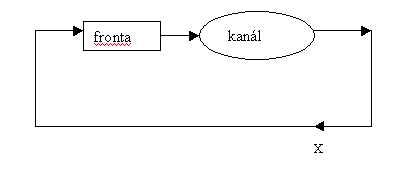
\includegraphics[width=0.7\linewidth]{net}
	\caption{Zadaná síť}
	\label{fig:net}
\end{figure}

\section*{Řešení}
V síti cirkulují 3 požadavky, jeden se vždy zpracovává a dva tedy musejí být ve frontě.

\paragraph{Zatížení kanálu obsluhy} = 1. \\
Kanál je neustále zatížen.

\paragraph{Střední délku fronty} = 2.

\paragraph{Pravděpodobnost, že délka fronty bude 1} = 0. \\
V síti jsou neustále 3 požadavky.

\paragraph{Průchodnost X} = $N(a , \sigma)$ \\
Plně závisí na propustnosti \emph{kanálu}.

\end{document}